% \guanzhi{The method feels slightly abstract in places. Can we give one concrete end-to-end example of the actual research loop? For example: the agent notices pin insertion fails due to unstable contact, inspects rollout videos + reward traces, modifies the algorithm, launches another evaluation, and compares the success rate against previous runs. A concrete instance would make the autonomous research process much easier to visualize.}

\section{Method}\label{sec: method}
In this section, we present a harness design that allows coding agents to perform automated research in the physical world. This procedure is decomposed into two stages: \emph{environment construction from human feedback} (\textbf{\texttt{{EN}}} in \method) and \emph{automatic policy improvement from real-world feedback} (\textbf{\texttt{{PIRE}}} in \method). 

% \begin{figure}
%     \centering
%     \includegraphics[width=1\linewidth]{corl_2026_template_submission/figures/agent-generate-env.pdf}
%     \caption{Enter Caption}
%     \label{fig:placeholder}
% \end{figure}

\subsection{Stage One: Environment Construction from Human Feedback}\label{sec:method-env}
For coding agents to conduct autonomous physical autoresearch, we need to first construct an agent-friendly abstraction of physical interaction and feedback as a structured environment. This includes task-specific safety constraints to support long-term operation, a real-time automated verification process for feedback and credit assignment, and a robust automatic reset mechanism to ensure fast iteration. To improve reliability, agents construct the environment APIs with procedural tool calls and refine their implementation according to human assessment. Human effort is a one-time cost that will be amortized across all implementations on all robots during subsequent automatic policy improvement in \cref{sec:method-tree}. 

\paragraph{Hard safety constraints} We restrict the configuration space and kinematic behaviors of the robot to a safe operational limit. The safety regions are sufficient for task completion and serve as hard constraints: violating these limits triggers an immediate task failure and an automated reset. This serves as a safeguard for real-world interaction, also as a source of episode termination or truncation.

\paragraph{Automated verification} 
During real-world experiments, robot learning needs real-time verification from sensor inputs to quantify experimental progress. To minimize human engineering efforts, coding agents are tasked with synthesizing a binary reward function from procedural tool calls to distinguish task outcomes. Given only a few minutes of success and failure demonstrations, the agents use the videos and proprioception recordings to maximize the prediction accuracy score while minimizing processing latency. For example, autoresearch discovers a robust reward function for pin insertion that is based on visual alignment, end-effector height, and force estimates. 
Coding agents also show their ability to design perception-dependent rewards in zip-tie insertion in \cref{fig:zip_tie_reward} and optimize its inference latency to under 150ms, which approaches the reactiveness of the human visual system~\citep{Thorpeetal1996}. More details are provided in the appendix. 
\begin{figure}[H]
    \centering
    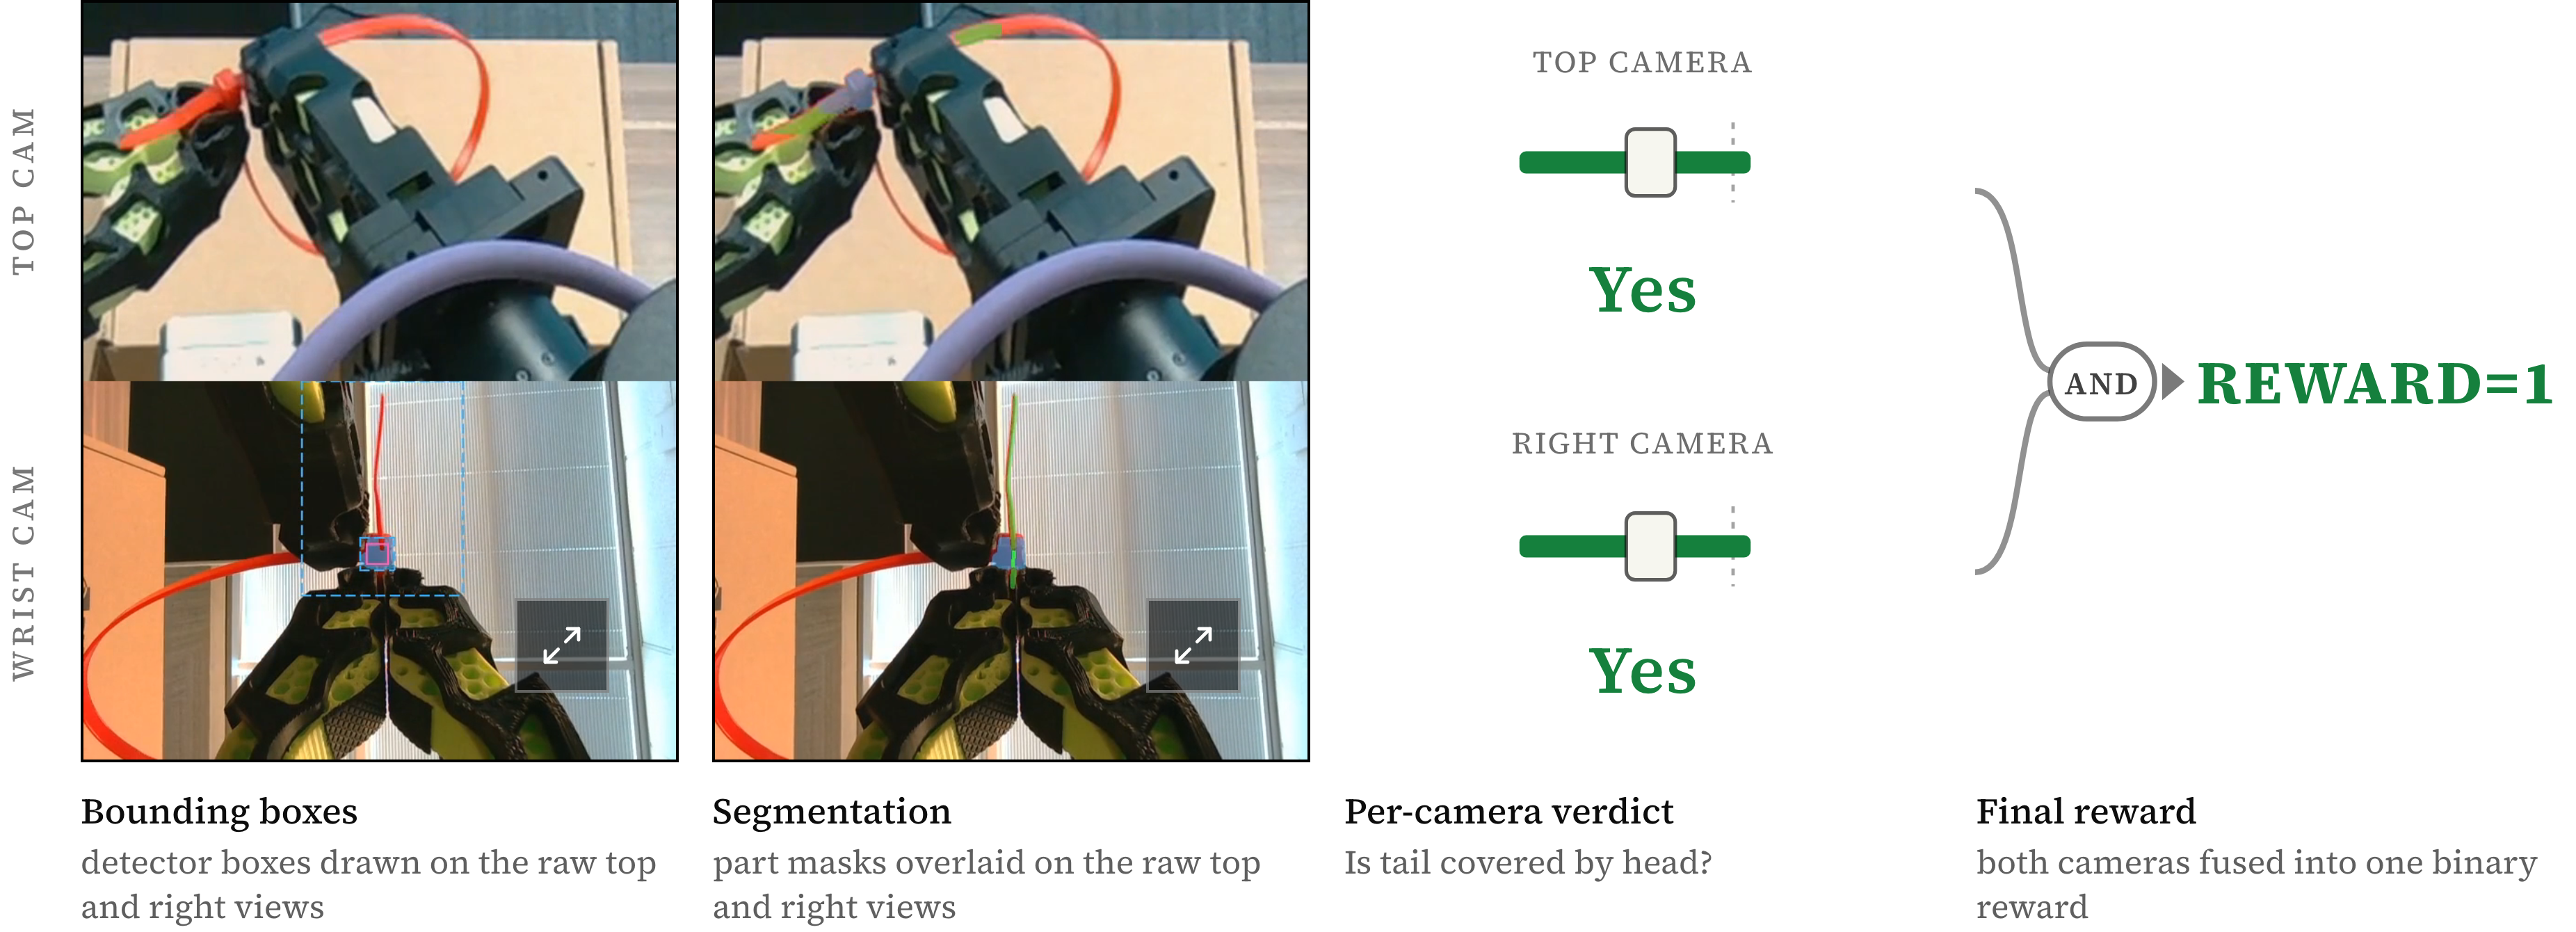
\includegraphics[width=0.95\linewidth]{ziptie_reward.png}
    \caption{Reward for zip-tie insertion. Cropping and image segmentation test whether the zip-tie strap passes through the zip-tie head. Two camera views are considered to prevent false positives.}
    \label{fig:zip_tie_reward}
\end{figure}


 
\paragraph{Automated reset}
Once a task is completed or fails, the agent executes a series of tool calls to restore the environment to its initial state. For contact-rich tasks, we employ procedural tool calls inspired by CaP-X~\citep{capx2026}, using modular manipulation skills to reset the environment directly to the start of the most challenging phase. By positioning the robot at the precise onset of critical actions, such as inserting a pin, seating a GPU, or grasping scissors, we strategically focus the learning system on these precision bottlenecks.

The safety constraints, automated verification, and automated reset constitute our Environment module (\textbf{\texttt{{EN}}} in \method). Policies also receive visual-proprioception sensor inputs and submit action commands to the robot controller, which, combined with our reward, constitutes the Rollout module (\textbf{\texttt{{R}}} in \method). Once constructed, coding agents have access to these modules through immutable Gym APIs~\citep{gym}, which provide feedback signals and debugging information for automated policy improvement. 

\subsection{Stage Two: Automated Policy Improvement from Real-World Feedback}\label{sec:method-tree}
The second stage leverages automated research to train a policy for a specific task. Upon initialization, the coding agent receives the task description with the ultimate objective of maximizing the task's success rate through autonomous experimentation. To achieve this, the agent is granted write permissions to a streamlined training codebase that supports basic end-to-end policy training and code-based policy synthesis. 
\vspace{-2mm}
\paragraph{A motivating example}
We illustrate this process using a pin insertion task, where the policy must insert a pin into a hole with a tight 4mm clearance (\cref{fig:overview}). During this automated research phase, the agent operates through a Policy Improvement module (\textbf{\texttt{{PI}}} in \method), where it reviews the literature to generate insights, formulates hypotheses, and directly modifies the training code---such as behavior cloning or RL algorithms---to optimize performance based on real-world automatic verification results. To gather rich evidence, the agent invokes environment APIs to log robot trajectories, video recordings, and reward signals during rollouts, and inspects these statistics to guide continued improvement. 

\vspace{-2mm}
\paragraph{Accelerating autoresearch via multi-agent scaling}\label{sec:method-fleet}
While automatic reset and verification mechanisms enhance the scalability of a single deployment loop, physical autoresearch can be further accelerated by launching a parallel, multi-agent decentralized collaboration protocol. This protocol deploys $N$ agents across $N$ physical robots to test $N$ hypotheses asynchronously. Each agent branches off from the same baseline policy training codebase, collaborating autonomously via Git to scale this Evolution module (\textbf{\texttt{{E}}} in \textbf{\texttt{{PIRE}}}). Without human intervention, agents spontaneously cherry-pick, copy, or merge successful training recipes from their peers to optimize their code search. Empirically, we observe that scaling the number of parallel agent-robot pairs drastically reduces the wall-clock time required to discover a high-success-rate policy recipe, as illustrated in Fig.~\ref{fig:real_pusht_pin_insertion}. 

To quantify how efficiently a coding agent converts its allocated physical resources into research progress, we propose two utilization metrics that complement task-level outcomes. Mean Robot Utilization (MRU) is the fraction of research wall-clock time during which the robot is actively executing an experiment. GPU utilization is the fraction of research wall-clock time during which the GPU is actively in use. 
A perfectly resource-saturated agent would push both metrics toward $1$; in practice, neither metric reaches this value for any frontier coding agent we evaluate. 
To measure how efficiently an agent team converts tokens into successful robot policies, we define Mean Token Utilization (MTU) as the fleet's average token consumption throughout autoresearch. We then calculate the token-to-success ratio to reflect the token efficiency of task learning. An empirical result of how robot and token utilization changes with agent team size is illustrated in Fig.~\ref{fig:utilization}. 


% \subsection{Stage Two: Automatic Policy Improvement from Real-world Feedback}\label{sec:method-tree}
% The second stage aims to use automatic research to train a policy for a specific task. At startup, the coding agent is presented with the task description. Its goal is to increase the success rate through automatic research. The coding agent has write-permission to a simple training codebase that supports basic end-to-end policy training and code-based policy synthesize. 
% \paragraph{A motivating example}
% We illustrate this process with our pin-insertion task, where policy inserts a pin into the hole which 4mm.
% % The environment is first co-designed by humans and agents. Agents can send actions to the robot and receive the resulting observation stream for policy execution. An agent can trigger an automatic rollout that runs until termination, which may be signaled by task success, task failure, or intervention by the safety module. The reward is then computed, and the robot is automatically reset to a random initial position. Agents have full access to the robot run logs, including rewards, observations, and executed actions, and can perform their own analysis on these data. Once this interface is fixed, we freeze the environment and begin the autoresearch phase. 
% During automated research, the agent reviews the literature to motivate ideas, formulate hypotheses, and validate them using empirical, real-world evaluation results. To gather high-fidelity evidence that grounds its reasoning, the agent invokes environment APIs to log robot trajectories, video recordings, and quantitative reward signals. Using these execution logs, the agent reasons over task outcomes, dynamically expanding or pruning its hypothesis space based on in-context real-world feedback. Throughout this iterative process, the agent maintains structured memory files and systematically monitors its research progress. 

% % \blue{Policy improvement module}
% % \blue{Evolution module}

% \paragraph{Accelerating Auto-Research through Multiagent Scaling}\label{sec:method-fleet}
% The automatic research progress is limited by the frequency of real-world experimental feedback. In order to accelerate this process, we design a multi-agent decentralized collaboration protocol that fans out $N$ agents on $N$ robots to test $N$ hypotheses asynchronously. 
% Each agent branches off from the same policy training codebase, and they are instructed to collaborate through git. Without further human guidance, agents can spontaneously copy or merge from other agents' training recipes to regulate their recipe searching. We observe that scaling the number of agent robots reduces the wall-clock time to discover the recipe for a high success rate. 

% refer to capX twitter teaser video
% For fleets of $N$ robots, \method launches $N$ independent agents in parallel---one per robot---each pursuing the same research goal under the policy-improvement loop of \ref{sec:method-tree}. The fleet setting multiplies the effective experiment budget, scaling the research throughput with $N$. Coordination is asynchronous and decentralized via a shared GitHub repository under version control. Each agent owns a branch and commits its code, configurations, logs, and verified components to it. Before launching its next candidate experiment, an agent can choose to reads peers' branches, avoids candidates already settled elsewhere, and steers toward underexplored directions of the shared research space. Version control supplies exactly the primitives a multi-agent research system needs: branches isolate parallel work, commits attribute each result to the agent that produced it, and the merged history serves as the fleet's persistent memory.
% straightforward, more general, not overclaim
% describe agent capability (literature review, logging task progress, exam experimental log, tool use, iterating on idea, monitor robot operation), see example in the appendix

% Once the environment is established, the agent will only be able to access its standard Gymnasium API while keeping its content frozen.  Necessary context about the task, including constraints and goal, will be provided. The agent mainly have access to modify all code under a repository that isolate it from pre-built environment. The environment interfaces and and physical tools usage API can provided. We integrate a toolkit of motion planning (CuRobo, PyRoki, etc) and visual grounding (AnyGrasp, SAM3, Gemini, etc), and wrapping functional tool usage into API. 


% \subsection{Accelerating Auto Research on Robot fleet}
% \label{sec:method-fleet}
% For fleets of $N$ robots, \method launches $N$ independent agents in parallel---one per robot---each pursuing the same research goal under the policy-improvement loop of \ref{sec:method-tree}. The fleet setting multiplies the effective experiment budget, scaling the research throughput with $N$. Coordination is asynchronous and decentralized via a shared GitHub repository under version control. Each agent owns a branch and commits its code, configurations, logs, and verified components to it. Before launching its next candidate experiment, an agent can choose to reads peers' branches, avoids candidates already settled elsewhere, and steers toward underexplored directions of the shared research space. Version control supplies exactly the primitives a multi-agent research system needs: branches isolate parallel work, commits attribute each result to the agent that produced it, and the merged history serves as the fleet's persistent memory.





% In this section, we characterize the extent to which the \textit{state-of-the-art} coding agent can conduct physical auto-research under proper harness loop.
% \method main consists of two agent harness stages: 1) Human-in-the-Loop environment construction. The agent is guided to build a verifiable reward from human feedback and autonomous reset pipeline calling physical tools. 2) Autonomous policy improvement via interative hypothesis reasoning and verification. Following CaP-X \citep{capx2026}, we implement computationally intensive perception and control primitives as stateless services (including but not limited to CuRobo, AnyGrasp, SAM3, and VDM such as Gemini) and provide APIs for agent to perform basic physical movement and understanding. We also showcase how our framework can be adopted to a multi-agent setting, in which we deploy a fleet of embodied agents to collaborate on a single research topic in a decentralized manner.



% \subsection{Agentic Environment Construction from Human Feedback}

% be specific and provide instance (zip-tie)
% Harness: Human provide examples (1 min data) rather than rule in text
% Wenli will have a figure (ZipTie reward)
% verifiable reward / score (source is the human)

% Instead of directly asking the agent for a performant policy, we harness the agent to establish a standard Gymnasium~\citep{gym} environment that bridges the gap between robot hardware and language model generated codes (LMPs) \citep{cap}. Stage 1 produces two key components: a reward function $r$ that scores robot observations for task completion, and a reset routine $\rho_0$ that returns the robot to a controlled initial state.  
% Additionally, the robot's control and sensing stack instantiates the observation and action spaces $(\mathcal{S},\mathcal{A})$, while the underlying dynamics includes real hardware do not have a closed form expression expressed in code. This process is the only human-in-the-loop step in \method and a one-time cost per task; through iterative dialog, the researcher guides the agent to design components of the environment, after which the research loop runs fully autonomously. 



% \paragraph{Verifiable Reward.}
% \tonghe{Not actually verifiable}
% The agent synthesizes a reward code that maps observations to a task feedback signal through the perception toolkit (e.g., estimating insertion depth or object pose). As a core component of credit assignment, an erroneous reward signal can silently invalidates every downstream experiment, thus we consider grounding and validating it against the available task specification---demonstrations, success/failure labels, and the natural-language goal---before deployment. 
% To efficiently automate the reward function design, we provide a set of labeled success and failure frames and have the agent calling external and internal tools to directly create LMP that optimizes classification accuracy. We found that this design minimizes human effort compared with providing hand-crafted rules as context. For instance, in the Zip-tie task, CodeX is able to generate a sophisticated reward function given only 1 minutes of teleoperation data with ground human label.
% As in \ref{img:}, the agent calls... \TODO{confirm details with Tonghe}
% The reward is later considered a fixed evaluation metric, ensuring that performance changes are attributable to the change of policy rather than to a shifting objective.


% \paragraph{Task-focusing reset.}
% The reset function reestablishes a controlled initial state between episodes and enables unattended, repeated trials. Beyond repetition, a well-chosen $\rho_0$ acts as a curriculum: by initializing each episode at the task bottleneck, it confines learning to the sub-skill that beyond the capability of classical control primitives. In pin insertion, grasping and transporting the pin are handled reliably by control primitives---grasp synthesis \citep{fang2023anygrasp} and motion planning \citep{curobo}---whereas high-precision insertion is not. The reset therefore, grasps the pin and positions it directly above the insertion site, so that online learning is devoted to acquiring the insertion behavior solely. Together, reward and reset convert bare hardware into a resettable, instrumented MDP in which autonomous self-improvement is well-posed.
